\section{Zielsetzung}
Ziel des Versuches ist es, die Funktionsweise des Franck-Hertz Versuches zu zeigen und 
die Energieniveaus von Quecksilber zu bestimmen.

\section{Theorie}
\label{sec:Theorie}
\section{Kosntruktion der ungestörten Franck-Hertz Kurve}
Eine Franck-Hertz Apperatur besteht aus einem evakuierten Gefäß das zum Beispiel Quecksilber enthält.
Abgebildet ist dies in Abbildung \ref{fig:Franck}.
\begin{figure}[H]
    \centering
    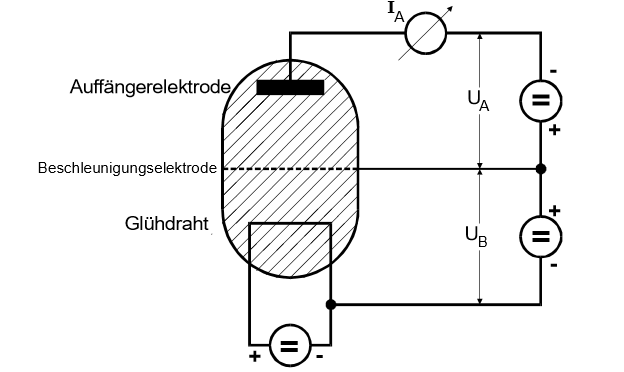
\includegraphics[width=10cm]{Bilder/Franck.png}
    \caption{Gezeigt wird ein schematisches Bild des Franck-Herz Versuches.}
    \label{fig:Franck}
\end{figure}
\noindent Beim Franck-Hertz Versuch werden die aus dem Glühdraht austretenden Elektronen durch die Spannungsdifferenz zwischen Glühdraht und Beschleunigungselektrode beschleunigt, bis sie die nötige kinetische Energie haben,
um ein Quecksilber Atom anzuregen.
Diese Elektronen können dabei elastisch oder inelastisch stoßen.
Bei einem elastischen Stoß ändert sich die Energie der gestoßenen Elektronen näherugsweise nicht, sondern nur die Richtung dieser.
Bis zu einer Energie von $E_{kin}=\increment E$ finden nur elastische Stöße statt.
Die Energie, die ein Elektron bei einem inelastischen Stoß abgibt, beträgt
\begin{equation}
    \increment E=E_1-E_0\frac{1}{2} m_0 \cdot v_{\symup{vor}}^2-\frac{1}{2} m_0 \cdot v_{\symup{nach}}^2 \. .
    \label{eqn:Energie}
\end{equation}
und entspricht der Energiediffferenz zwischen dem Grundzustand eines Hüllenelektrons von Quecksilber zum ersten angeregten Zustand.
Dabei emmitiert das Quecksilber-Atom beim zurückkehren in den Grundzustand ein Photon mit der Energie
\begin{equation}
    h \cdot \frac{c}{\lambda}= \increment E \. .
    \label{eqn:Wellenlänge}
\end{equation}
Hier wird die Gegenfeldmethode benutzt, um die Energie der schnellsten Elektronen zu bestimmen.
Es wird zwischen Beschleunigerelektrode und Auffängerelektrode eine Gegenspannung $U_A$ angelegt.
Nach der Beschleunigung haben die Elektronen die Energie
\begin{equation}
    \frac{1}{2} m_0 \cdot v_{\symup{vor}}^2=e_0 U_B
    \label{eqn:Beschleunigung}
\end{equation}
und durch das Gegenfeld werden nur die Elektron mit
\begin{equation}
    \frac{1}{2} m_0 \cdot v_{z}^2 \>= e_0 U_A
    \label{eqn:Gegenspannung}
\end{equation}
gemessen.
Ab einer Energie von $E_{kin}=\increment E$ ist ein Elektron in der Lage, ein Quecksilber Atom anzuregen.
Damit finden auch inelastische Stöße ab, und die Elektronen geben ihre Energie an die Quecksilber-Atome am Ende der Franck-Hertz Röhre ab.
Mit steigender Beschleunigungsspannung verschiebt sich der Ort des inelastischen Stoßes in der Röhre nach vorne, und die Elektronen erhalten nach dem Stoß immer mehr kinetische Energie.
Dadurch wird wieder die Grenze erreicht, ab der die Ungleichung \ref{eqn:Gegenspannung} erfüllt wird und wieder Elektronen gemessen werden.
Dies steigt dann immer weiter an, da mit steigender Spannung jetzt auch die Elektronen, die sich nicht vollständig in z-Richtung bewegen, die Auffängerelektrode treffen.
Mit weiter steigendem $U_B$ wird dann wieder die Anregungsenergie des Quecksilbers erreicht, sodass die Elektronen zwei inelastische Stöße durchführen können.
Dies wiederholt sich bei steigender Beschleunigungsspannung immer wieder.
Nun kann noch mit einbezogen wird, dass die Beschleunigung immer größer wird, sodass die Elektronen bei einer höheren Beschleunigungsspannung schneller auf die Elektrode auftreffen.
Damit ist allgemein ein globaler Anstieg des gemessenen Stroms messbar, jedoch nach Formel \ref{eqn:Gegenspannung} eben nur in dem Bereich in dem auch Strom gemessen werden kann-
Nach diesen Erkentnissen wird die Kurve in Abbildung \ref{fig:Theorie} für die Abhängigkeit vom Auffängerstrom $I_A$ zu $U_B$ erwartet.

\begin{figure}[H]
    \centering
    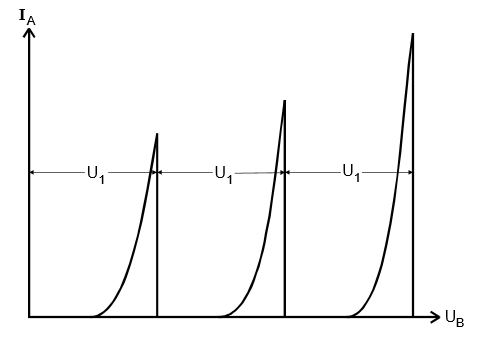
\includegraphics[width=10cm]{Bilder/Theorie.png}
    \caption{Abgebildet ist der erwartete Verlauf vom Auffängerstrom zur Beschleunigungsspannung beim Franck-Hertz Versuch.}
    \label{fig:Theorie}
\end{figure}

\noindent Dabei entspricht $U_1$ mit
\begin{equation}
    U_1=\frac{1}{e_0}(E_1-E_0)
    \label{eqn:Abstand}
\end{equation}
\noindent Dem Abstand der Maxina beziehungsweise der spontanen Abfälle, also den Punkten, ab denen gerade $E_{kin}=\increment E$ gilt.

\subsection{Störungen der Franck-Hertz Kurve}
Störungsquellen sind das Kontaktpotential, das Spektrum der Elektronen, der Dampfdruck und mögliche andere Übergänge des Hüllenelektrons.
Das Kontaktpotential wird mit
\begin{equation}
    K=\frac{1}{e_0}(\phi_B-\phi_G)
    \label{eqn:Kontaktpotential}
\end{equation}
berechnet, wobei $\phi_G$ der Austrittsarbeit des Glühdrates und $\phi_B$ der Austrittsarbeit der Beschleunigungselektrode entspricht.
Durch die Differenuz beider Austrittsarbeiten ist das tatsächlich auf die Elektronen wirkende Potential anders, als die eingestellte Beschleunigungsspannung.
Dies resultiert dann in einer Verschiebung der Franck-Hertz Kurve auf der x-Achse.\\
Die Energie der aus dem Glühdraht austretenden Elektronen ist nicht gleichverteilt, sondern unterliegt einer Fermi-Dirac-Verteilung.
Das führt dazu, dass die inelastischen Stöße bei dem Versuch nicht alle zur selben Beschleunigungsspannung auftreten, sondern zu geringfügig unterschiedlichen.
Daher werden die Peaks in der Franck-Hertz Kurve abgerundet und niedriger.
Zudem wird der instantane Abfall zu einer stetig fallenden Funktion, die an die Steigung vor dem nächsten Peak anknüpft.\\
Der Dampfdruck ist insofern relevant, dass die Peaks des Franck-Hertz Versuches nur dann erkennbar sind, wenn ein Elektron, sobald es die Anregungsenergie von Quecksilber erreicht, auch auf ein Quecksilber Atom trifft.
Dies ist jedoch nicht gewährleistet, wenn der Dampfdruck zu niedrig und nicht genügend Quecksilber-Atome vorhanden sind.
Dann können die Elektronen höhere Energien erreichen, die groß genug sind, um andere Anregungszustände von Quecksilber zu treffen.
Und wenn der Dampfdruck zu hoch ist, treten sehr viele elastische Stöße auf, sodass es immer weniger Elektronen gibt, die auf die Auffängerelektrode treffen.
Der optimale Dampfdruck, der Sättigungsdampfdruck, kann mit 
\begin{equation}
   p_{\textrm{sät}} =\frac{2.9\cdot10^{-4}}{\bar{w}}
    \label{eqn:Sättigungsdampfdruck}
\end{equation}
berechnet werden.
Dabei ist $\bar{w}$ die mittlere freie Weglänge der Elektronen, die um einen Faktor von 1000 bis 4000 kleiner als a sein sollte, damit die Stoßwahrscheinlichleint ausreichend ist.
Aus dem Sättigungsdampfdruck lässt sich mit 
\begin{equation}
    p_{\textrm{sät}}(T)=5.5 \cdot 10^4 \exp(-6876/T)
    \label{eqn:Temperatur}
\end{equation}
der Zusammenhang mit der Temperatur beschreiben.

\cite{V601}

